%\documentclass[aspectratio=43]{beamer}
\documentclass[t]{beamer}
\usetheme{ffmodern}  %% Themenwahl

\usepackage[ngerman]{babel}
\usepackage[T1]{fontenc}    % richtige Silbentrennung
\usepackage[utf8]{inputenc} % Umlaute etc.!
\usepackage{eurosym}
\usepackage{tikz}
\usepackage{pgffor}
\usepackage{textcomp}
\usepackage{textpos}
\usepackage{tikz}
\usepackage{mathtools}
\usepackage{grid-system}

\usetikzlibrary{arrows,decorations.pathmorphing,backgrounds,fit,positioning,shapes.symbols,chains}

%-----------------
\title{Freifunk}
\author{Das freie WLAN-Netz} % TODO: anderer Untertitel? Bürgernetz?
\date{22. Juli 2016}
\license{CC-BY-3.0}

\begin{document}
  \maketitle

  %-----------------
  \begin{frame}{Was ist Freifunk?}

    % TODO: Überarbeiten (mit Icons)
    \begin{itemize}
      \item Initiative für freie (Funk-)Netze
      \item Mitmachnetz: Netz in Nutzerhand
      \item Offen für jeden, als Nutzer oder Betreiber
      \item Nicht kommerziell
      \item Krisensichere Kommunikation
    \end{itemize}
  \end{frame}

  %-----------------
  \begin{frame}{Was ist Freifunk?}
    \begin{center}
      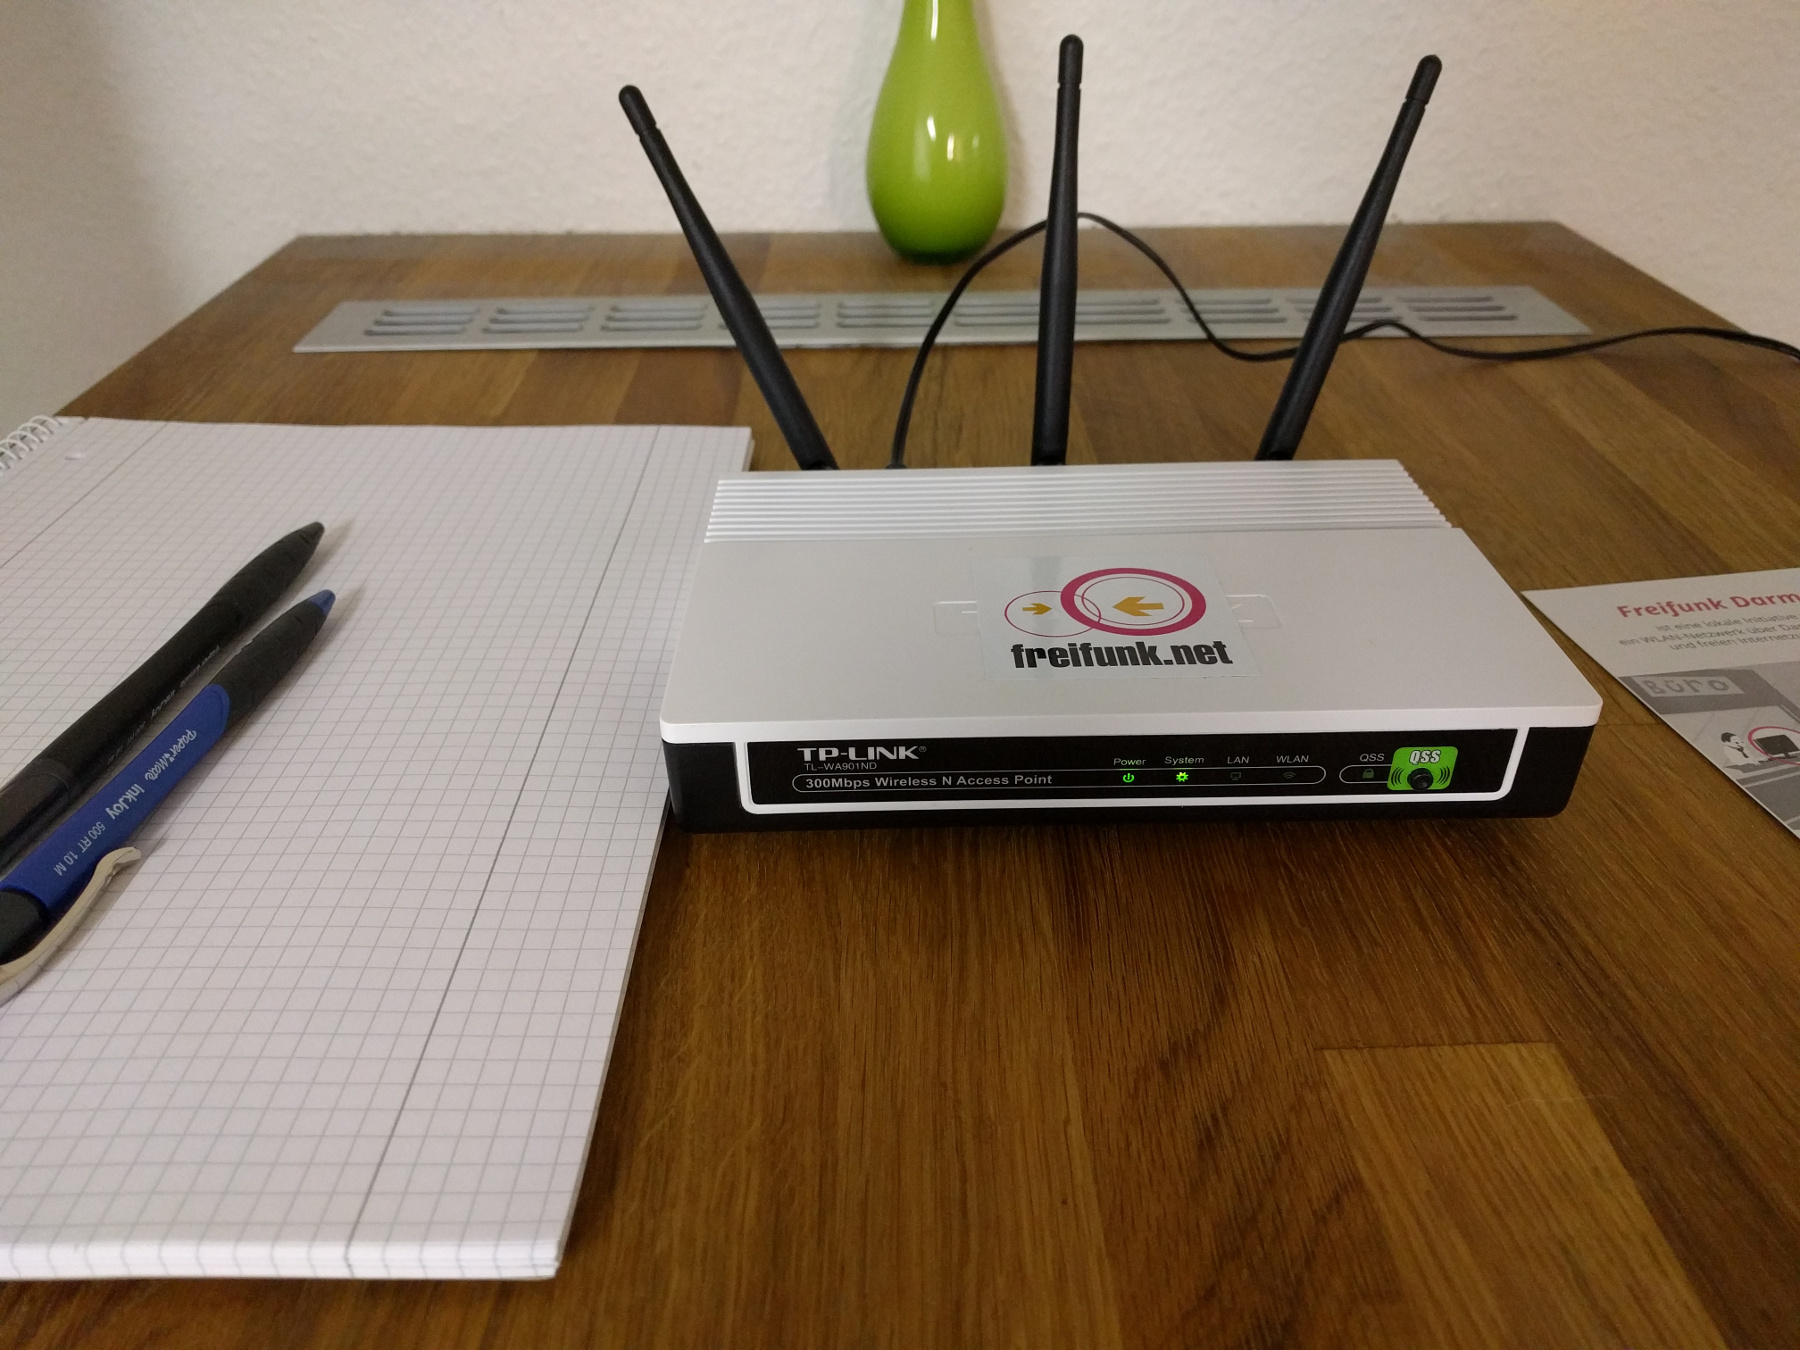
\includegraphics[width=7cm]{images/homerouter}
    \end{center}
  \end{frame}

  %-----------------
  \foreach \index in {1, ..., 3, 5}
  {
    \begin{frame}{Das Netzwerk}
      \centering \includegraphics[width=9cm]{images/network_\index}
    \end{frame}
  }

  %-----------------
  \begin{frame}{Verbreitung}
    \begin{columns}
      \begin{column}{0.6\textwidth}
        \begin{itemize}
          \item Deutschlandweit über  \href{http://freifunk.net/wie-mache-ich-mit/community-finden/}{350 lokale Gruppen}
          \item mehr als 37.700 offene Zugangspunkte
          % TODO: Zahlen auf den aktuellen Stand bringen

        \end{itemize}
      \end{column}
      \begin{column}{0.4\textwidth}
        \begin{center}
          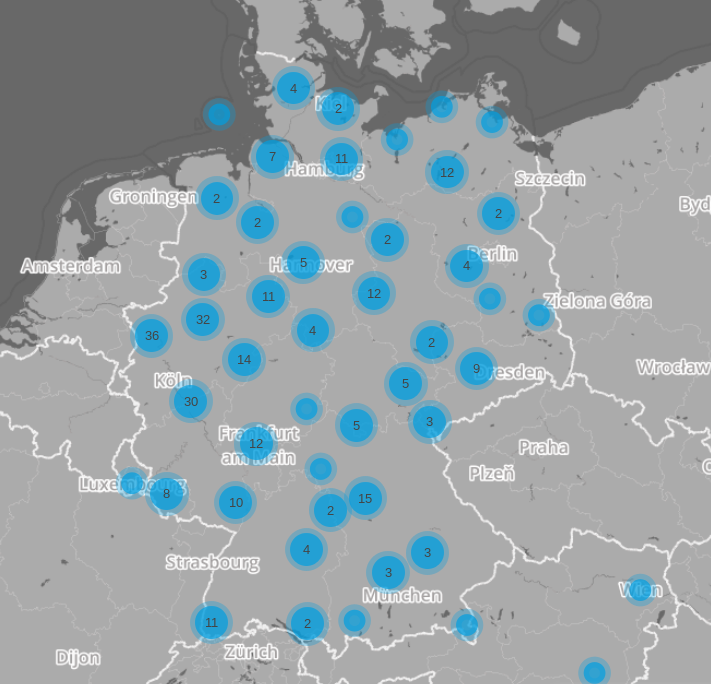
\includegraphics[width=\textwidth]{images/2016-06-01_map-de}
        \end{center}
      \end{column}
    \end{columns}
  \end{frame}

  \begin{frame}{Ziele von Freifunk}
    \begin{itemize}
      \item \textbf{Verständnis} von Kommunikationsnetzen fördern $\xRightarrow{}$ Bildungsauftrag
      \item Beteiligung der Bevölkerung an \textbf{Forschung, Aufbau und Entwicklung} dezentraler Netze
      \item Beteilung an gesellschaftlichen Initiativen, um die \textbf{Verbreitung freier Netze} zu unterstützen
    \end{itemize}
  \end{frame}


  %-----------------
  \begin{frame}{Freifunk Darmstadt}
    \begin{itemize}
      \item Initiative des Chaos Darmstadt e.V.
      \item Über 480 Freifunk-Router in Darmstadt und Umgebung
      \item Täglich über 1000 Nutzer gleichzeitig online
      %\item Ermöglicht durch eine starke Freifunk-Community mit großem ehrenamtlichen Einsatz
    \end{itemize}
  \end{frame}

  %-----------------
  \begin{frame}{Stadt Darmstadt}
    \begin{itemize}
      \item September 2015: Kooperation mit OB Partsch, Stadt Darmstadt vereinbart
      \item Bis Weihnachten wurden alle angefragten Unterkünfte mit WLAN versorgt
      \item Großartige Zusammenarbeit mit ASB, DRK, Feuerwehr und der städtischen IT
      \item IT Materialkosten < 5.000 \texteuro
    \end{itemize}
  \end{frame}

  \begin{frame}{Babenhausen – 4 Monate Freifunk}
    \begin{center}
      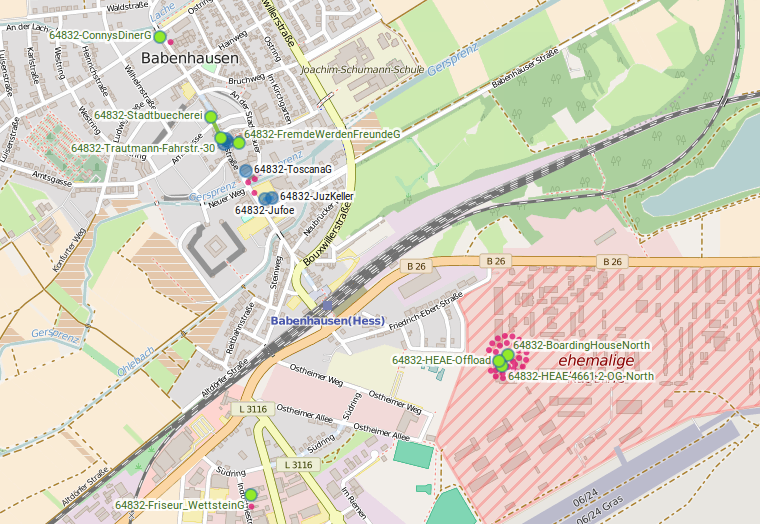
\includegraphics[width=0.9\textwidth]{images/2016-07-21-babenhausen}
    \end{center}
  \end{frame}

  %-----------------
  \begin{frame}{Störerhaftung}
    \begin{itemize}
      \item Keine Haftung für Knotenbetreiber
      \item Internetverkehr geht über unsere Gateways. Haftungsbefreiung nach TMG \S8.
      \item Wir nehmen die gesetzlichen Vorschriften wörtlich: Wir sammeln keine Daten.
    \end{itemize}
  \end{frame}

  %-----------------
  \begin{frame}{Richtfunknetz}
    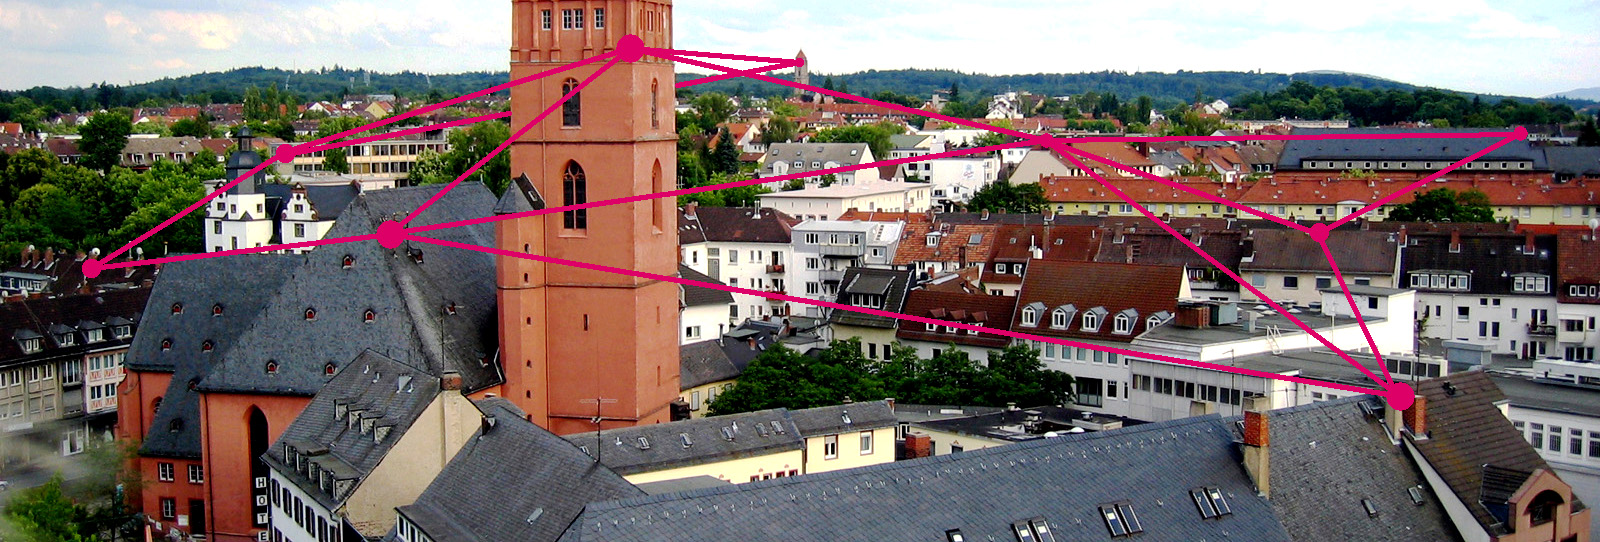
\includegraphics[width=\textwidth]{images/banner-stadtkirche-darmstadt}
    \begin{columns}
      \begin{column}{0.65\textwidth}
        \begin{itemize}
          \item Eigene Infrastruktur
          \begin{itemize}
            \item Redundanz und Lastverteilung
            \item Unabhängig vom Internet
          \end{itemize}
        \end{itemize}
      \end{column}
      \begin{column}{0.25\textwidth}
        \begin{center}
          \vspace{-1.5cm}
          \hspace{-0.75cm}
          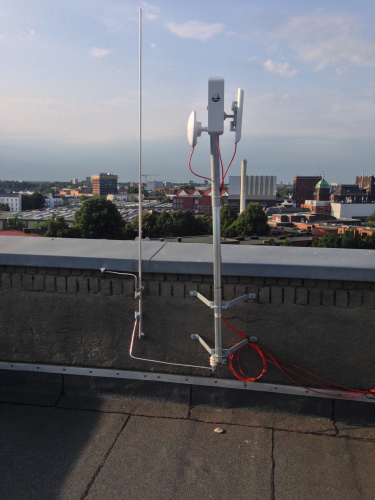
\includegraphics[width=\textwidth]{images/hamburg-richtfunkmast}
        \end{center}
      \end{column}
    \end{columns}
  \end{frame}


  \begin{frame}{Richtfunknetz}
    \leavevmode\makebox(0,-165){\put(5,-60){
      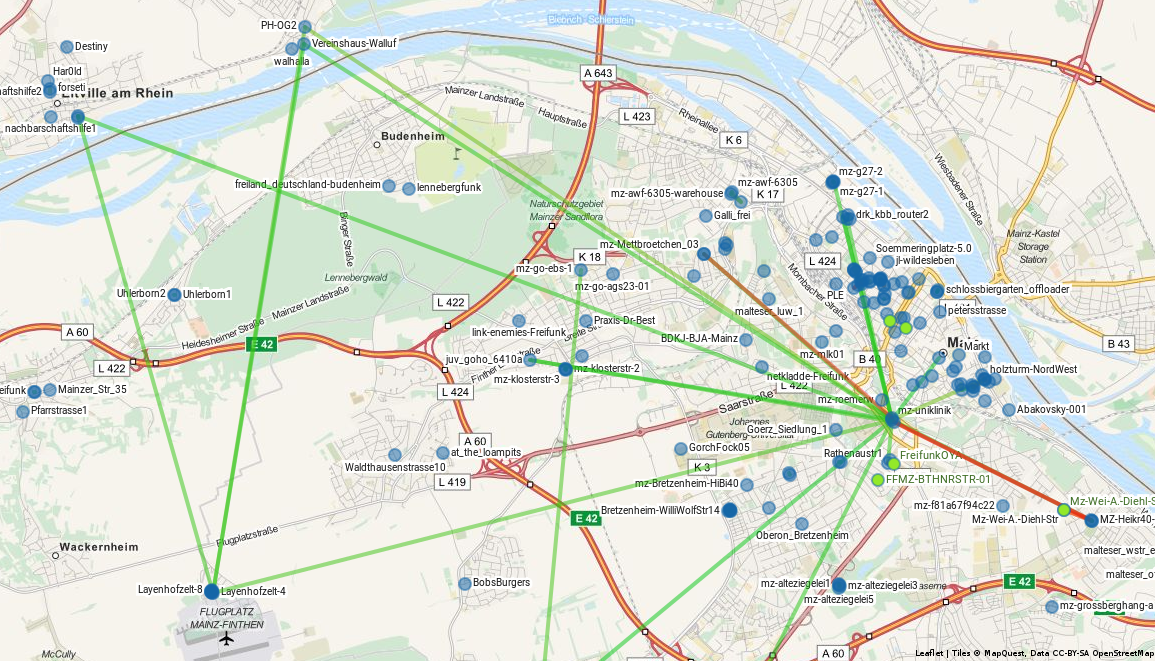
\includegraphics[width=0.95\textwidth]{images/2016-06-12_map-mainz-rifu}
    }}
    \pause
    \leavevmode\makebox(0,-165){\put(2.3,-60){
    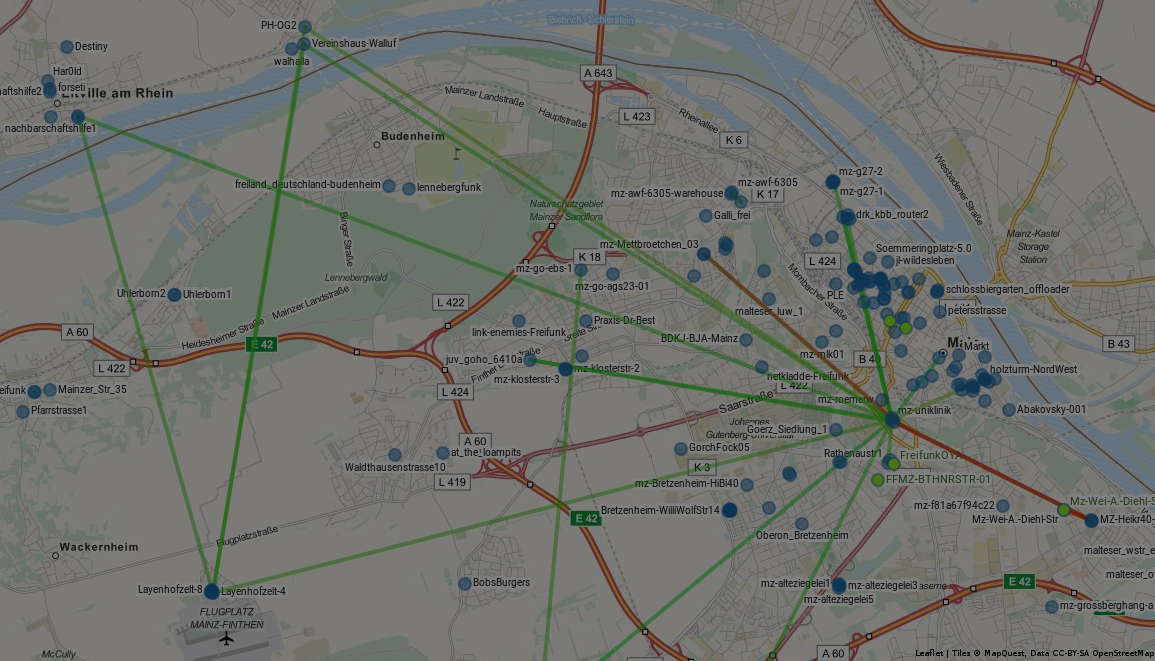
\includegraphics[width=0.95\textwidth]{images/2016-06-12_map-mainz-rifu-dark}
    }}
    \leavevmode\makebox(0,-165){\put(160,0){
      \includegraphics[height=0.75\textheight]{images/2016-08-06_malchen.jpg}
    }}
  \end{frame}

  %-----------------
  \begin{frame}{Freifunk lebt vom Mitmachen}
    \begin{itemize}
      \item Freifunk ist \textbf{kein Dienstleister}
      \item Aufbau einer \textbf{lokalen Community} (falls nicht vorhanden) wünschenswert
      \item Andere Freifunk-Gruppen helfen gerne dabei und \textbf{geben Wissen weiter}
    \end{itemize}
  \end{frame}

  %-----------------
  \begin{frame}
    \huge
    \vspace{3em}
    \center
    Freifunk für Geflüchtete!
  \end{frame}


  \begin{frame}{Groß-Gerau}
    \center
    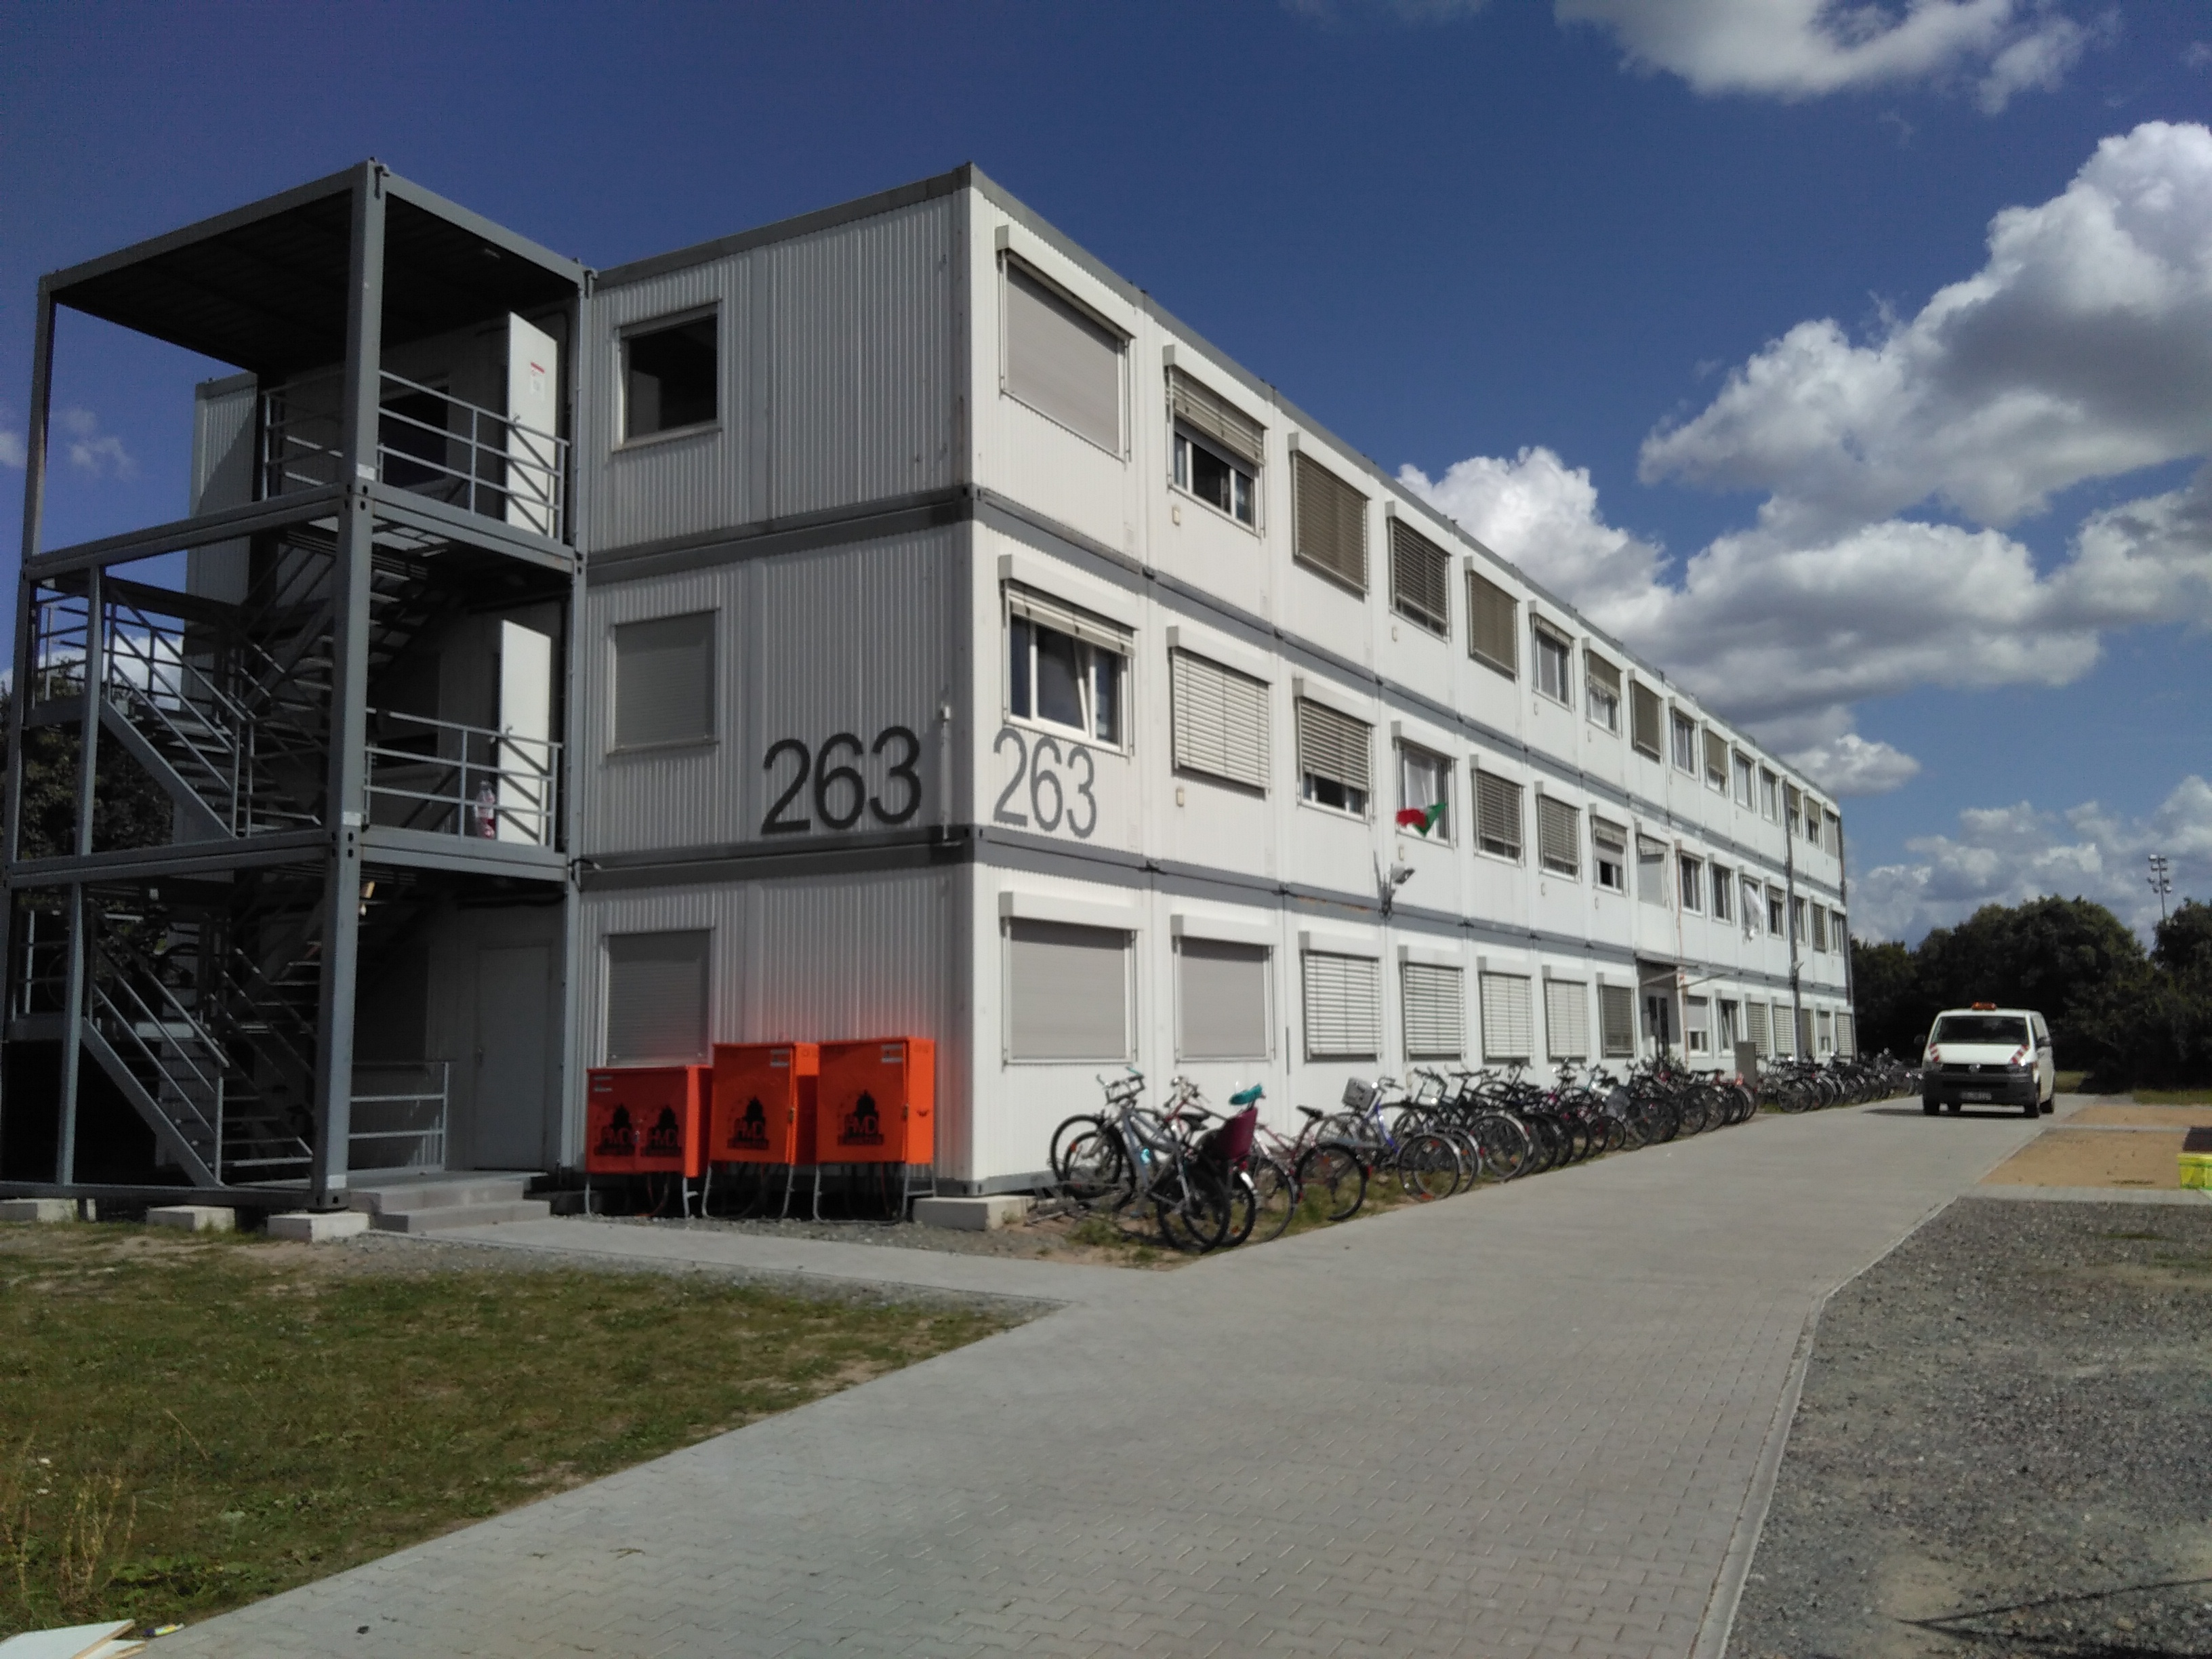
\includegraphics[height=0.75\textheight]{images/2016-08-08_ggsportpark.jpg}
  \end{frame}

  \begin{frame}{Riedstadt-Goddelau}
    \center
    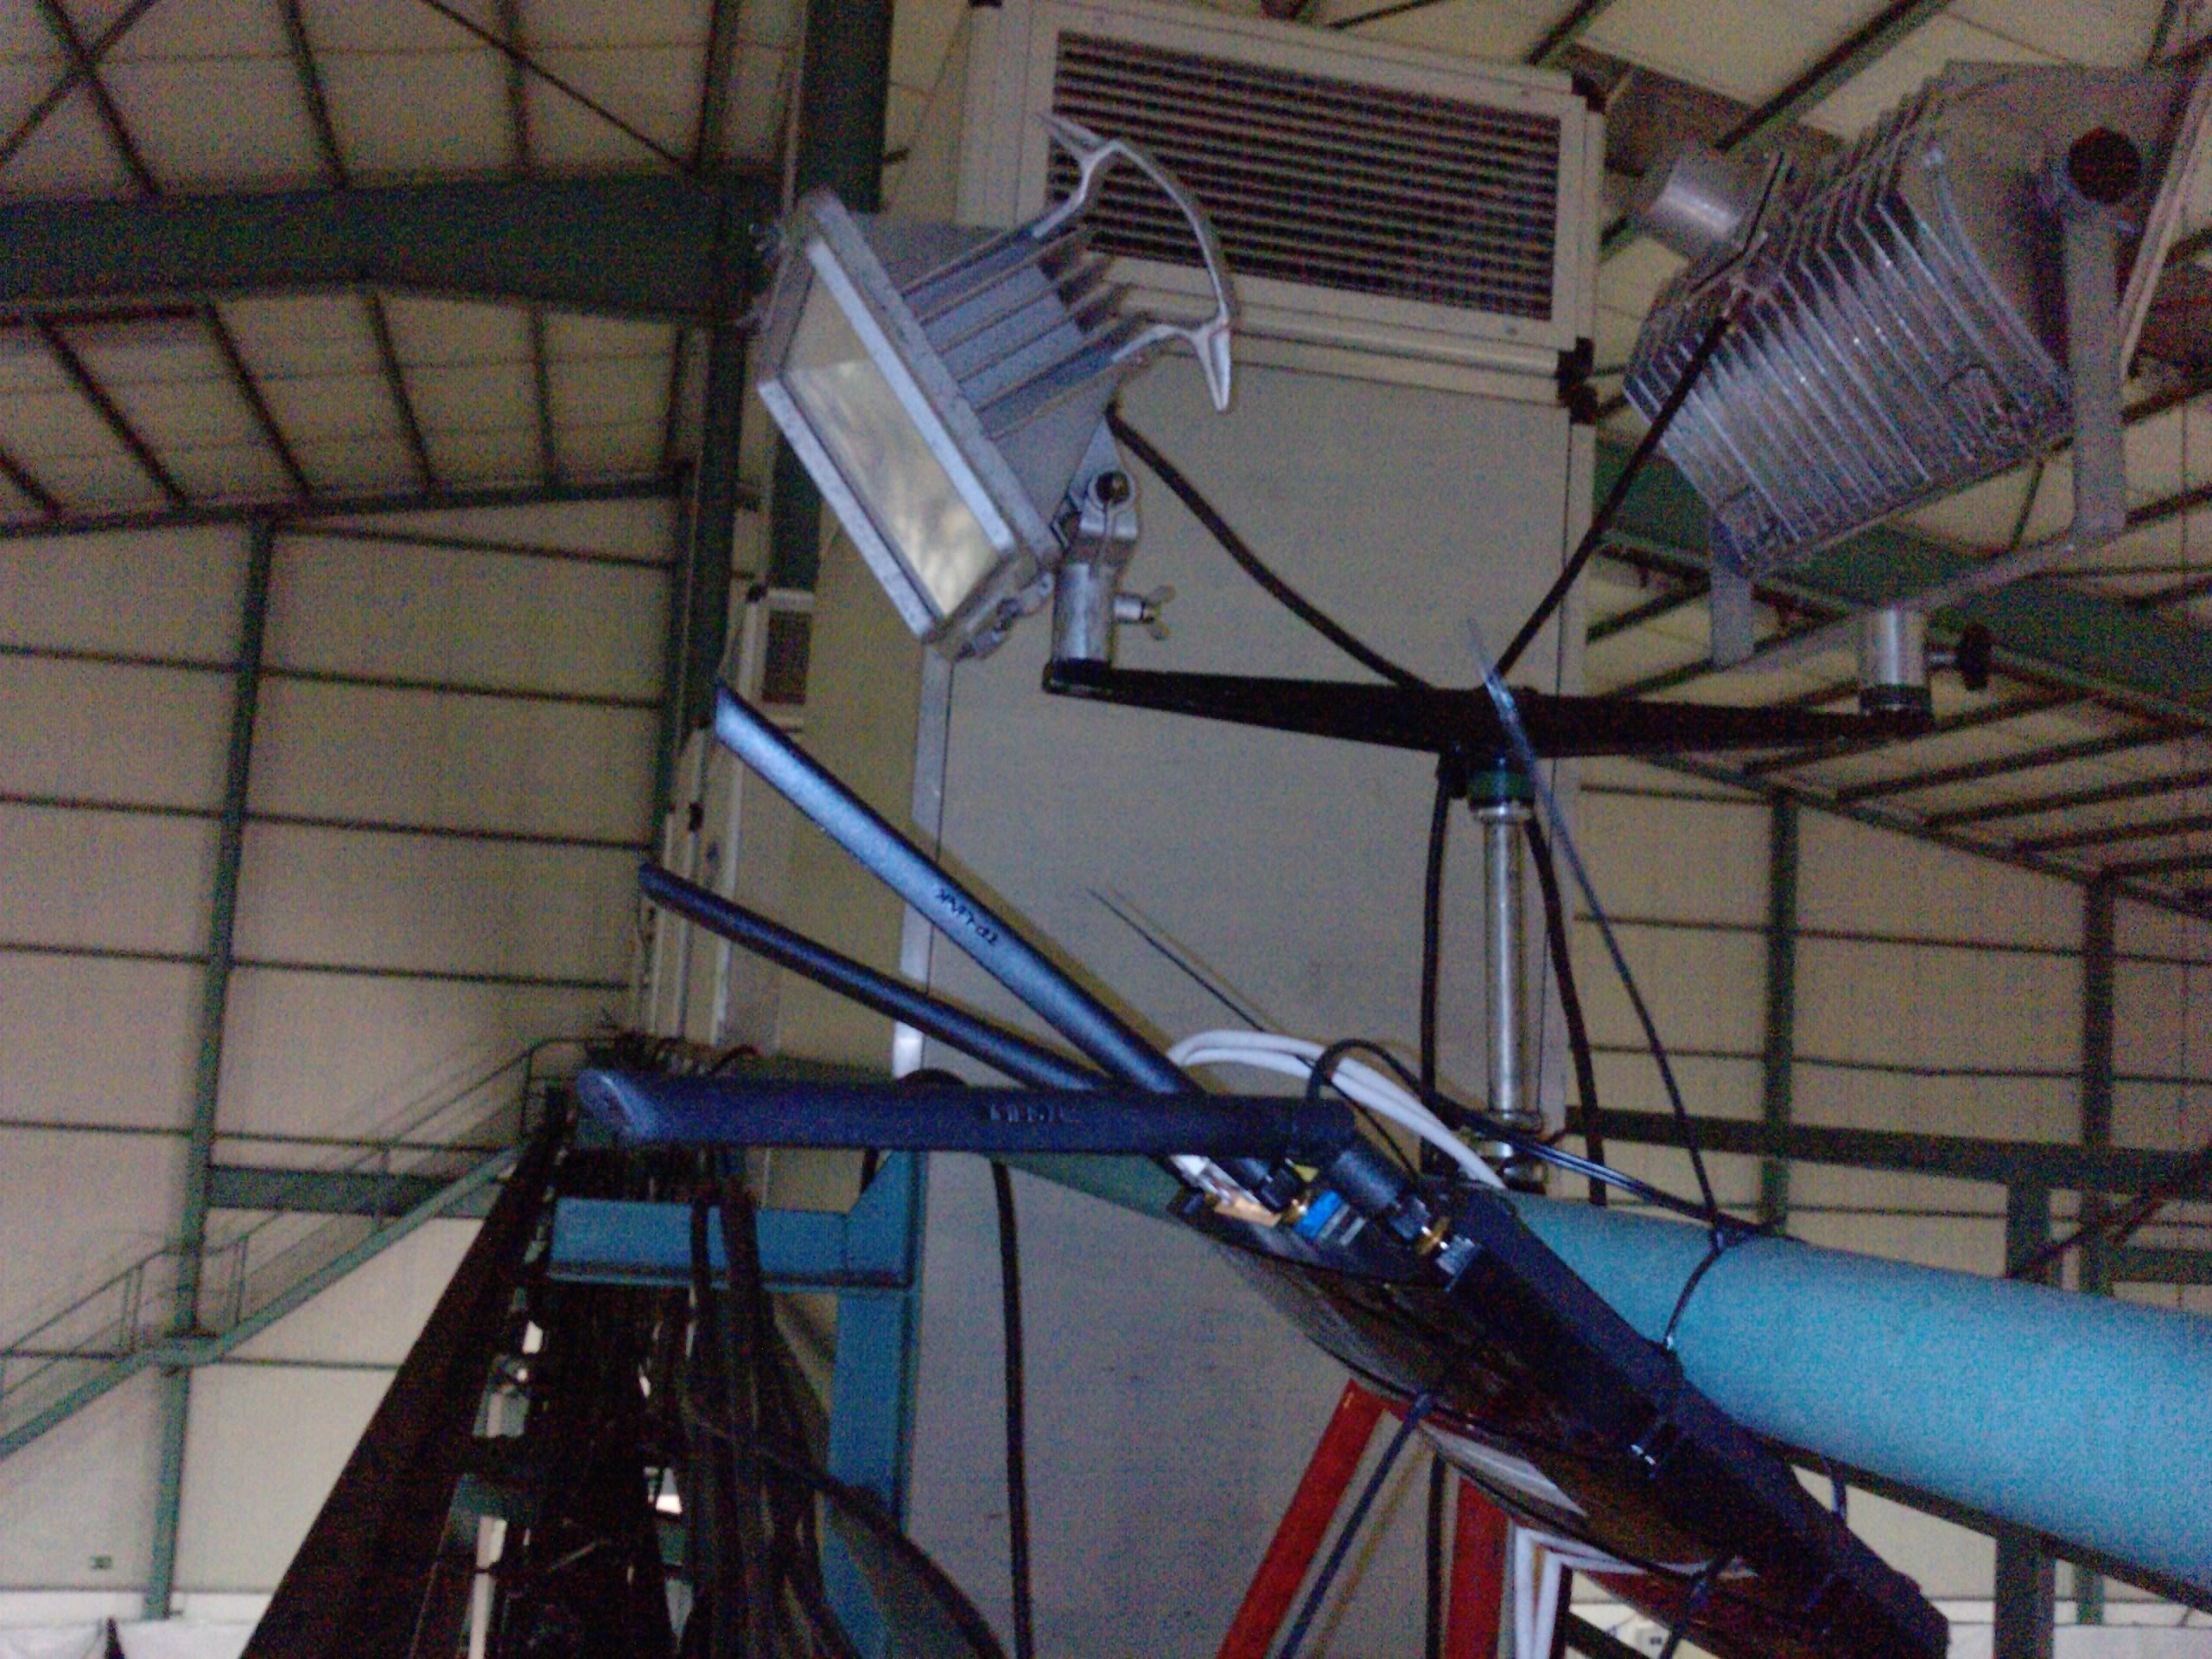
\includegraphics[height=0.75\textheight]{images/heae-goddelau-traeger.jpg}
  \end{frame}

  \begin{frame}{Stockstadt}
    \center
    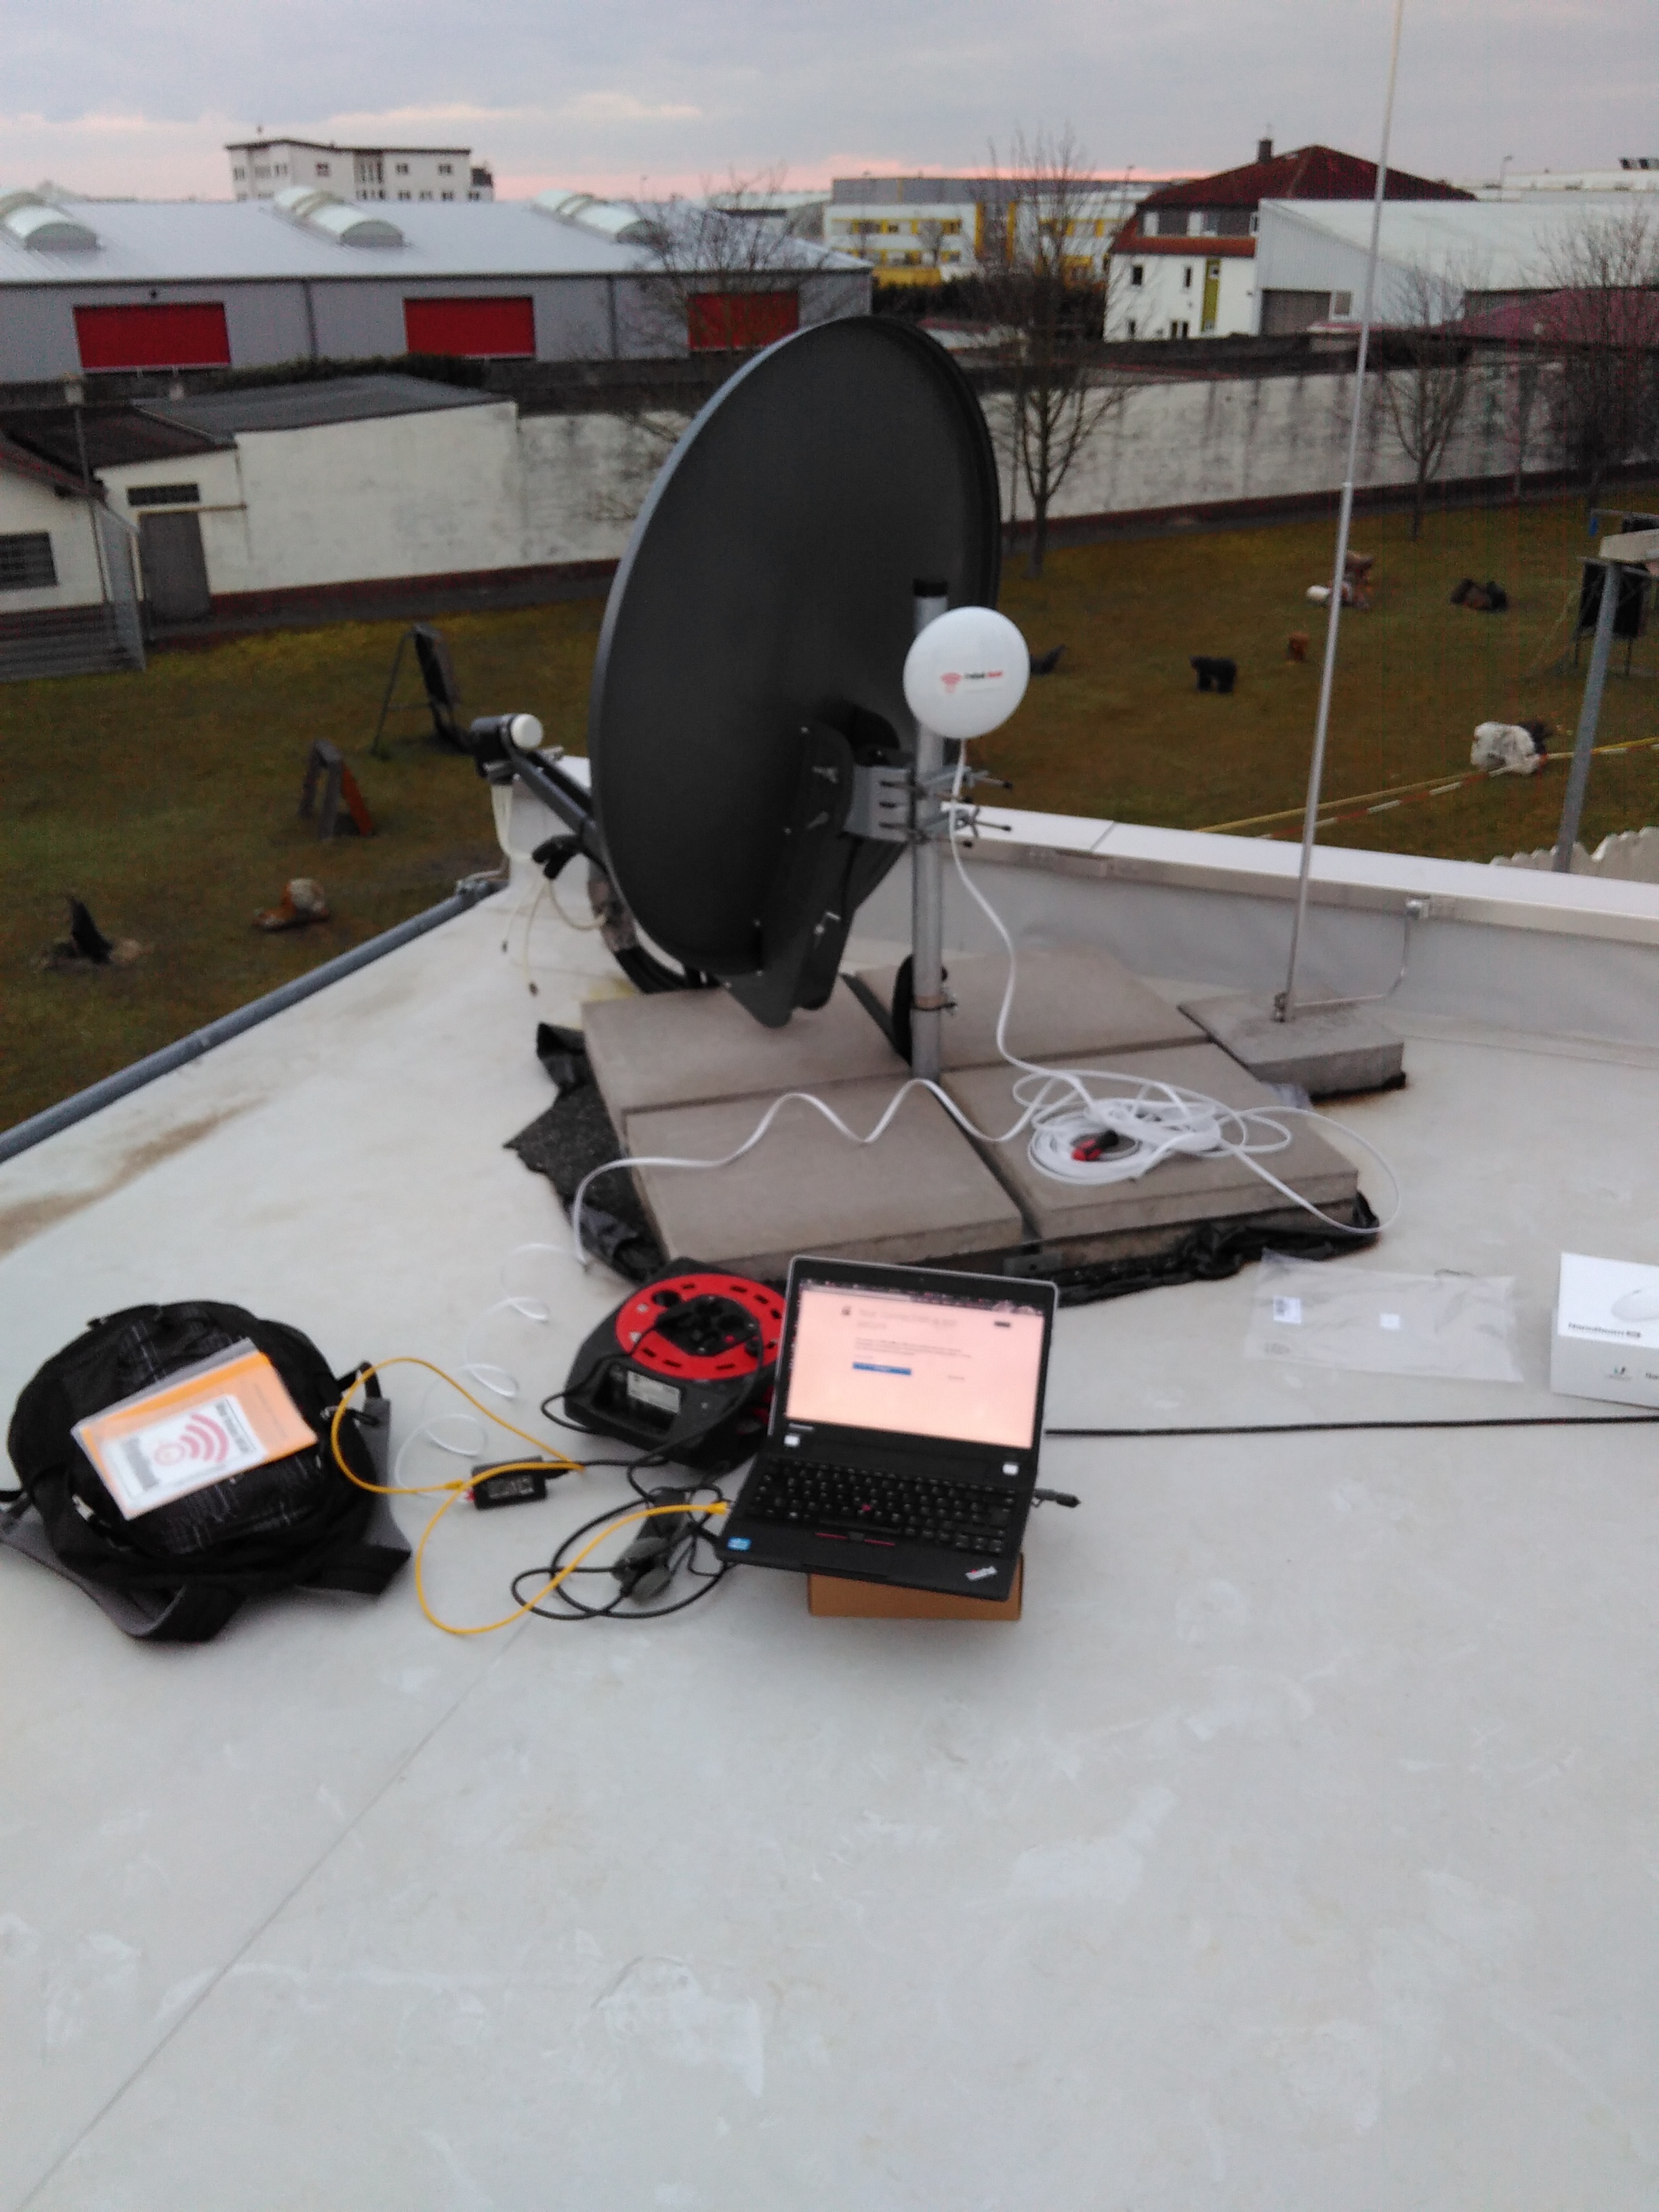
\includegraphics[height=0.75\textheight]{images/unterkunft-stockstadt-dach.jpg}
  \end{frame}

  \begin{frame}{Stockstadt}
    \center
    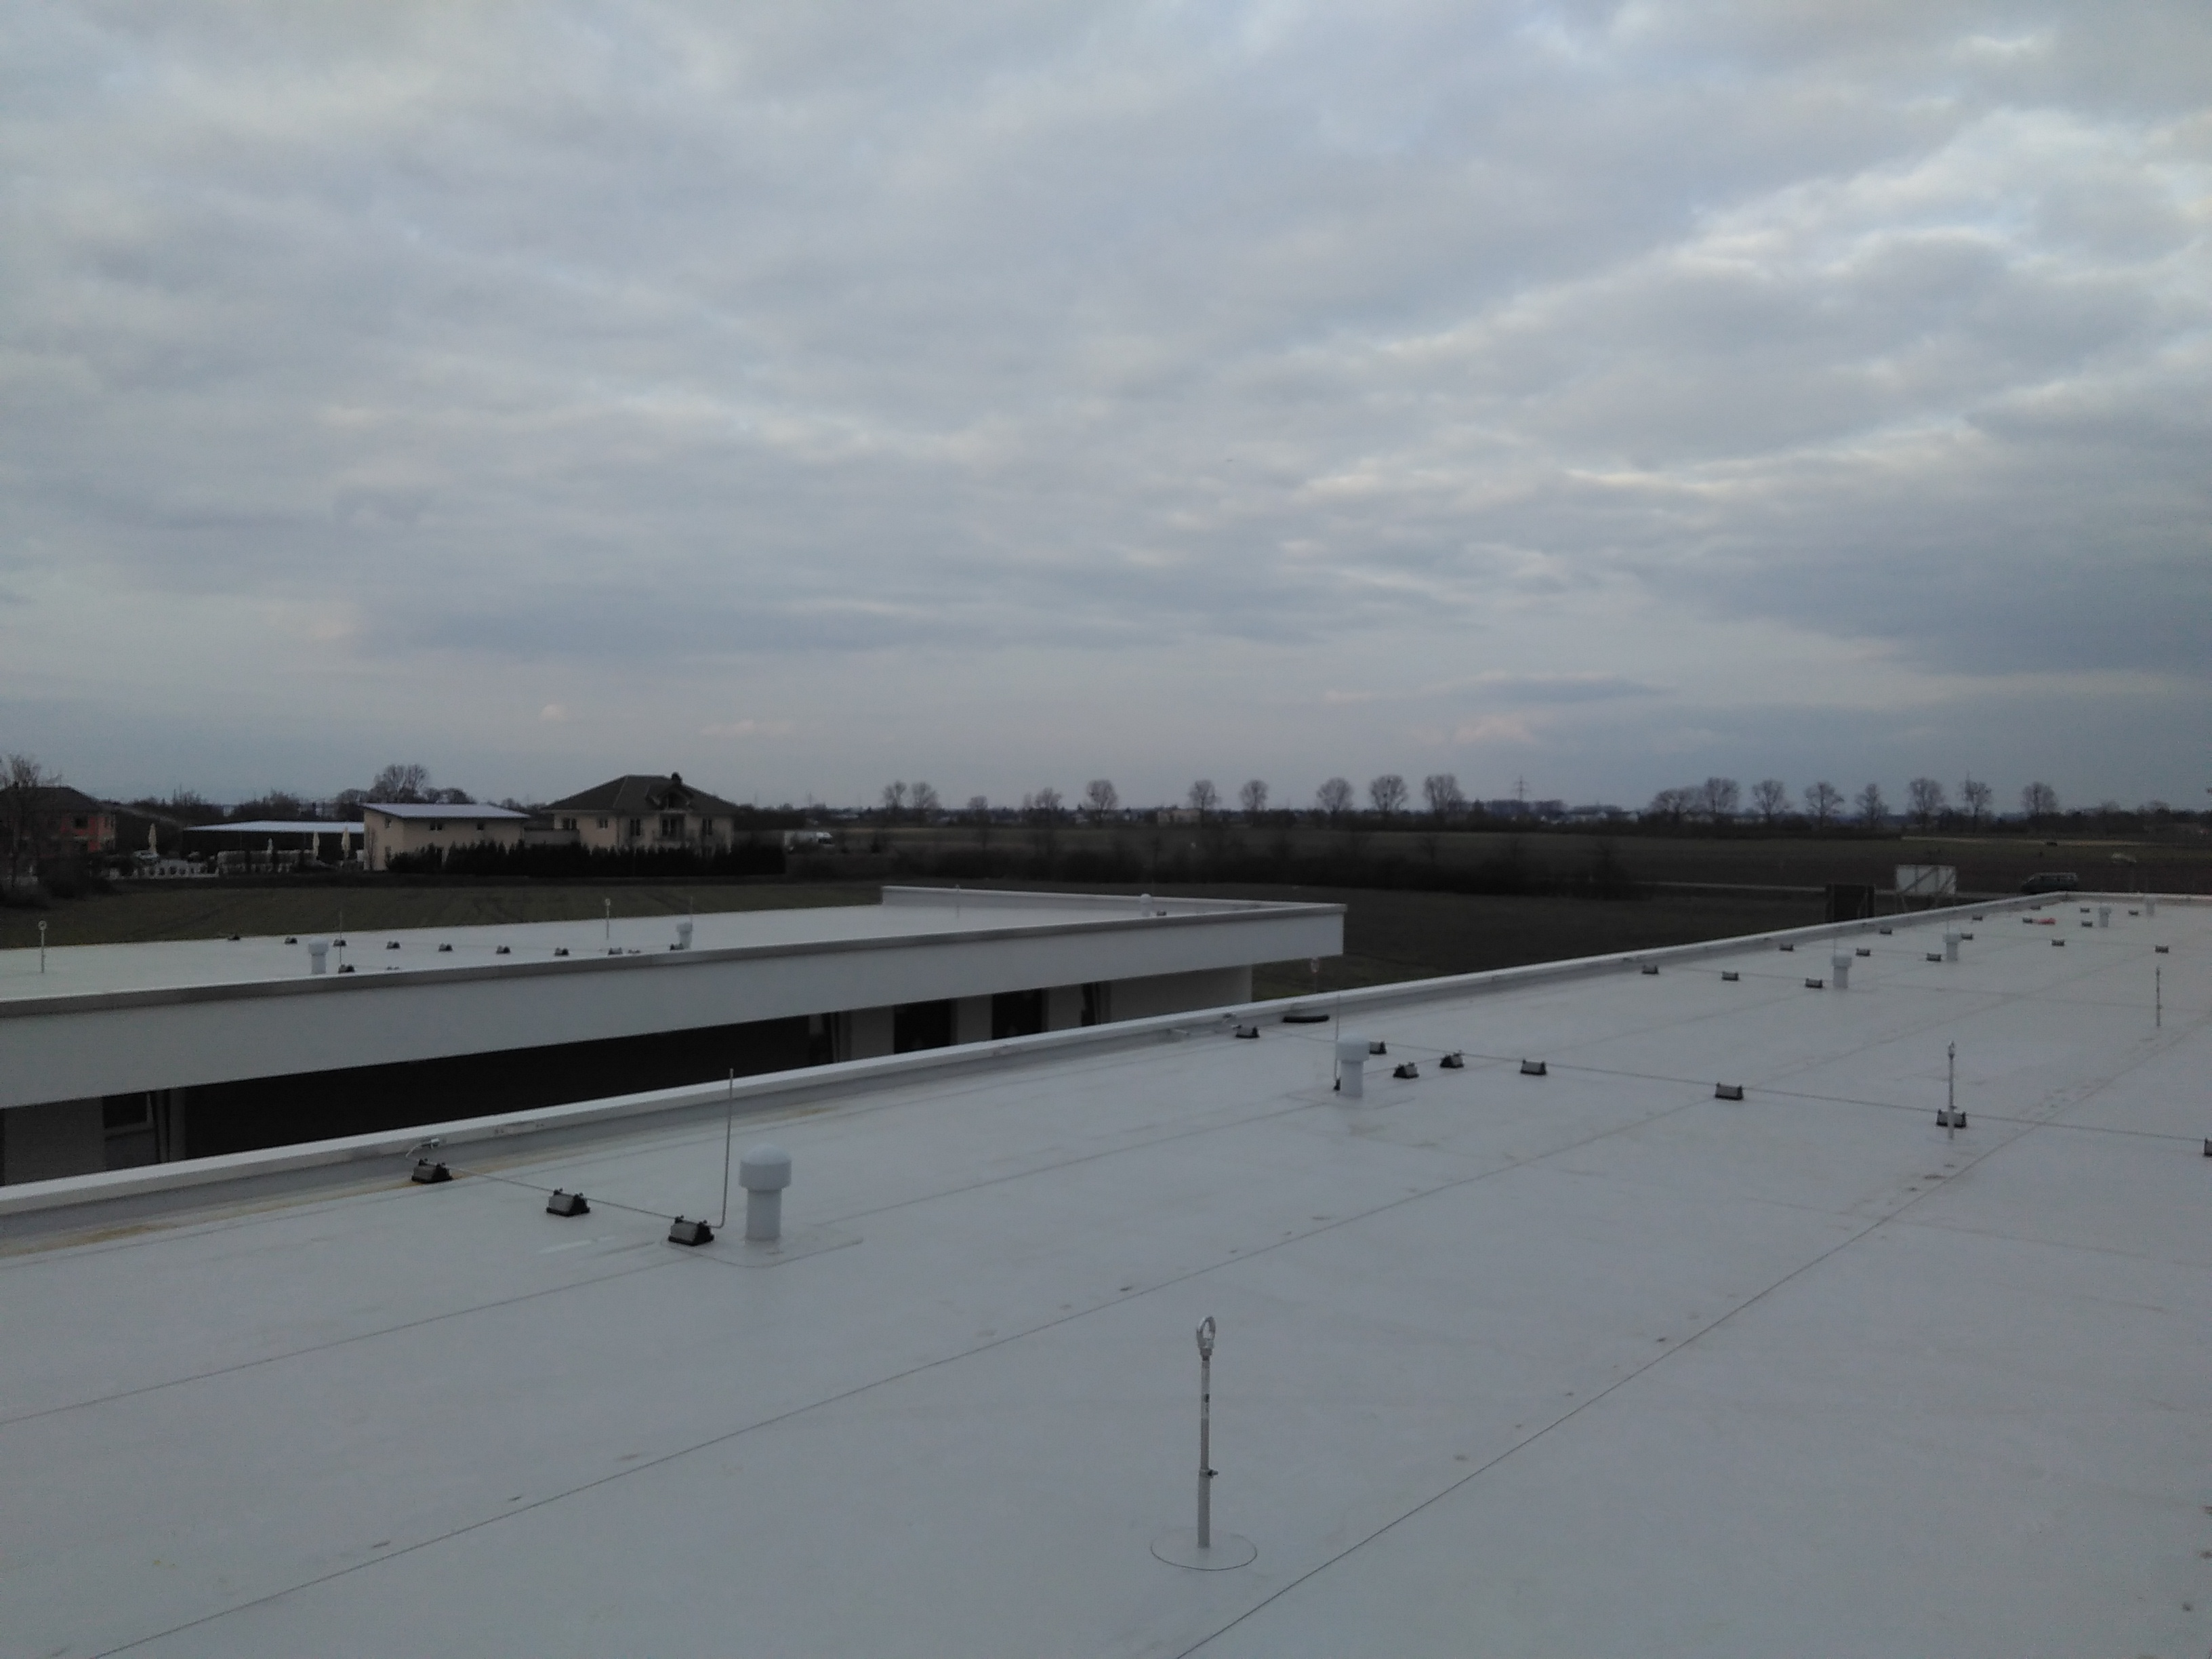
\includegraphics[height=0.75\textheight]{images/unterkunft-stockstadt-dach-aussicht.jpg}
  \end{frame}

  \begin{frame}{In 6 Schritten zum Freifunk-Netz}
    \begin{itemize}
      \pause
      \item Allgemeine Infos zur Unterkunft sammeln: Betreiber, Mieter, ...
      \pause
      \item Woher kommt das Freifunk-Netz?
      \pause
      \item Wer finanziert den Aufbau?
      \pause
      \item Kontakt zur Freifunk-Community
      \pause
      \item Konkrete Detailplanung zusammen mit dem Betreiber
      \pause
      \item Aufbau
    \end{itemize}
  \end{frame}

  %-----------------

  \begin{frame}{Vielen Dank!}
    \begin{textblock*}{0cm}(\textwidth-2cm,-2cm)
      \begin{figure}[h]
        \def\svgwidth{2.5cm}
        \input{logo.pdf_tex}
      \end{figure}
    \end{textblock*}
    \begin{itemize}
      \item Freifunk Darmstadt
      \begin{itemize}
        \item Webseite: \href{http://darmstadt.freifunk.net/}{darmstadt.freifunk.net}
        \item E-Mail: info@darmstadt.freifunk.net
        \item Treffen: Jeden Montag um 18:30 Uhr
      \end{itemize}
      \vspace{1em}
      \item Liste aller Communities auf \href{https://freifunk.net/}{freifunk.net}
    \end{itemize}
  \end{frame}
\end{document}
